\newpage
%===================================================================
\section{Transient Effects}\label{sec:4d}
%===================================================================

\subsection{Experimental principle}\label{sec:transient_theory}
When the RF is modulated on and off, the competition between optical
pumping (rate $P$) and collisional/RF relaxation (rate $R$) drives the
dark-state population toward its steady value with a first-order
exponential law, $n_2(t) = n_2(\infty) - [n_2(\infty)-n_2(0)]e^{-t/\tau_{\mathrm{eff}}}$,
where $\tau_{\mathrm{eff}}^{-1} = P + R$ (Eq.~2G-14 of
Ref.~\cite{OpticalPumpingRubidium2002}). The RF-off half-period therefore
gives the pure optical-pumping time constant $\tau_p$, whereas the moment
the RF is switched on the pumped spin ensemble undergoes coherent
precession about $B_{\mathrm{rf}}$ in the rotating frame, producing
damped Rabi oscillations in the transmitted light (Eqs.~2G-15/16) with
period $T = 1/(\gamma B_{\mathrm{rf}})$. The buffer gas (Ne) slows
diffusion to the cell walls so that $R$ is dominated by intrinsic spin
relaxation rather than wall-quenching, extending $\tau_{\mathrm{eff}}$
into the range accessible with a kHz-scale square-wave envelope.

\subsection{Settings}
A \SI{90}{\kilo\hertz} RF magnetic field, perpendicular to the static
Zeeman field, was amplitude-modulated with a \SI{5}{\hertz} square wave
(0--5\,V) from an AFG-2225 function generator. The square-wave gate was
recorded on CH1 and the photodetector voltage on CH2 as in
Section~\ref{sec:common_procedure}. The sweep field was tuned to bring
the static Zeeman splitting into resonance with the \SI{90}{\kilo\hertz}
RF for each isotope separately. Three peak-to-peak RF voltages
($V_{\mathrm{pp}} = 1,\,2,\,3\,\mathrm{V}$) were used for both $^{85}$Rb
and $^{87}$Rb, yielding six data sets analysed identically; the
$^{85}$Rb, $V_{\mathrm{pp}}=\SI{2}{\volt}$ run is used as the
representative example below.

\subsection{Raw time-domain signal}
Figure~\ref{fig:ch1_ch2_85_2vpp} shows a typical oscilloscope trace. Each
modulation period contains an \emph{optical-pumping recovery} (hatched):
when the RF is off, $\sigma^+$ D$_1$ light progressively pumps atoms into
the $m_F=F$ dark state and the transmitted intensity rises exponentially;
a \emph{ringing} interval (cross-hatched) immediately after the RF is
switched back on, where coherent Rabi oscillations appear as a damped
sinusoidal modulation; and a \emph{steady state} (remaining intervals)
where pumping and RF-driven depumping balance dynamically.

\begin{figure}[ht]
  \centering
  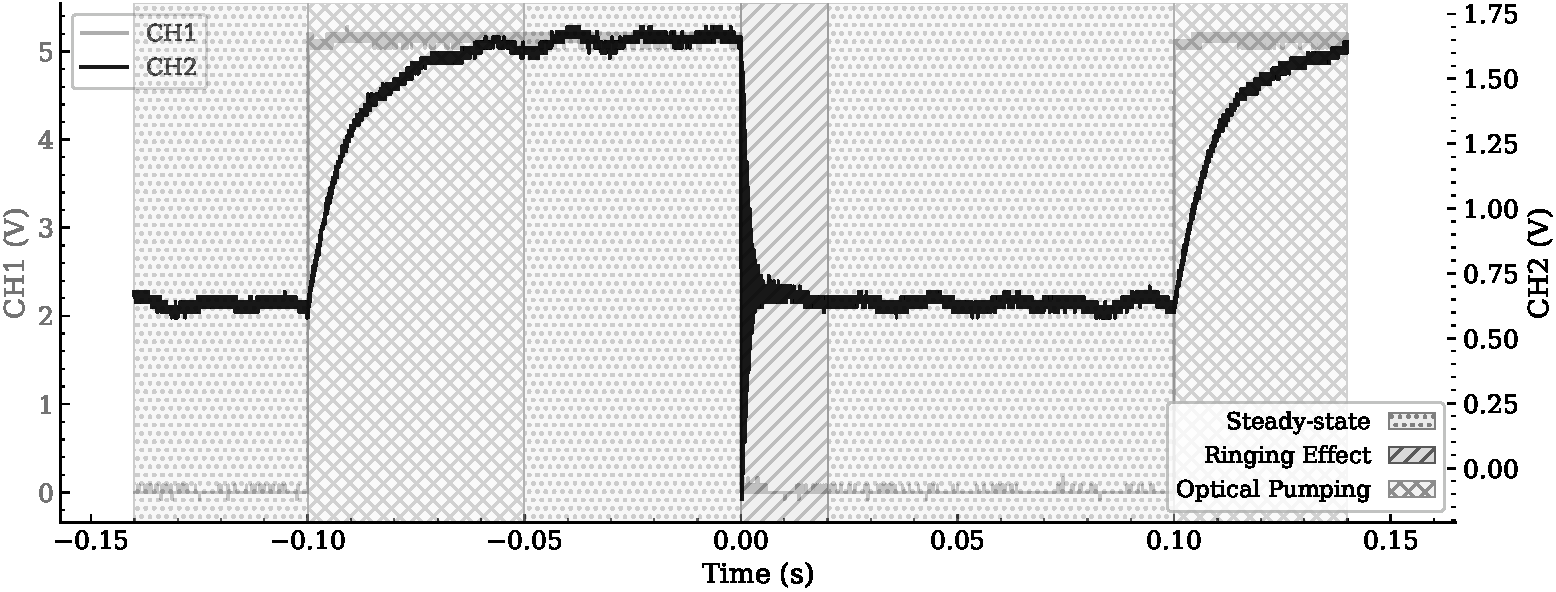
\includegraphics[width=0.85\linewidth]{figures/4d_CH1_and_CH2_vs_Time_85_2VPP.pdf}
  \caption{Oscilloscope traces of the RF control signal (CH1) and
    transmitted light intensity (CH2) for $^{85}$Rb at
    $V_{\mathrm{pp}} = \SI{2}{\volt}$. Hatched: optical-pumping interval;
    cross-hatched: ringing interval.}
  \label{fig:ch1_ch2_85_2vpp}
\end{figure}

\subsection{Steady-state noise analysis}\label{sec:fft}
A discrete Fourier transform of three concatenated steady-state segments
of CH2 ($t \in [-0.14,-0.10]\,\mathrm{s}$, $[-0.05,0]\,\mathrm{s}$, and
$[0.02,0.10]\,\mathrm{s}$, each DC-subtracted and zero-padded for
resolution) exhibits a dominant peak near \SI{60}{\hertz} consistent with
AC-mains pickup (see
\texttt{figures/4d\_CH2\_Spectrum\_Concatenated\_Hz.pdf}). Since the
ringing of interest sits two orders of magnitude higher (kHz range), no
digital filtering was applied.

\subsection{Optical pumping time constant \texorpdfstring{$\tau_p$}{tau\_p}}\label{sec:tau_p}
The RF-off half-period ($t \in [-0.10,0]\,\mathrm{s}$) was fit to
\begin{equation}
  I(t) = C - A\,e^{-t/\tau_p},
  \label{eq:op_model}
\end{equation}
with $C$ the fully-pumped saturation level, $A = C - I_{\min}$ the
initial deficit, and $\tau_p$ the pumping time constant. After
time-origin shifting ($t_{\mathrm{start}}=0$) for numerical stability, a
Levenberg--Marquardt non-linear least squares fit
(\texttt{scipy.optimize.curve\_fit}, seeded at $C \approx \max I$,
$A \approx \max I - \min I$, $\tau_p \approx \SI{20}{\milli\second}$)
yielded the parameters with their $1\sigma$ covariance-diagonal
uncertainties. Residuals were inspected to verify the single-exponential
adequacy; Fig.~\ref{fig:optical_pumping} shows the fits and residuals
for both isotopes at $V_{\mathrm{pp}} = \SI{2}{\volt}$.

\begin{figure}[ht]
  \centering
  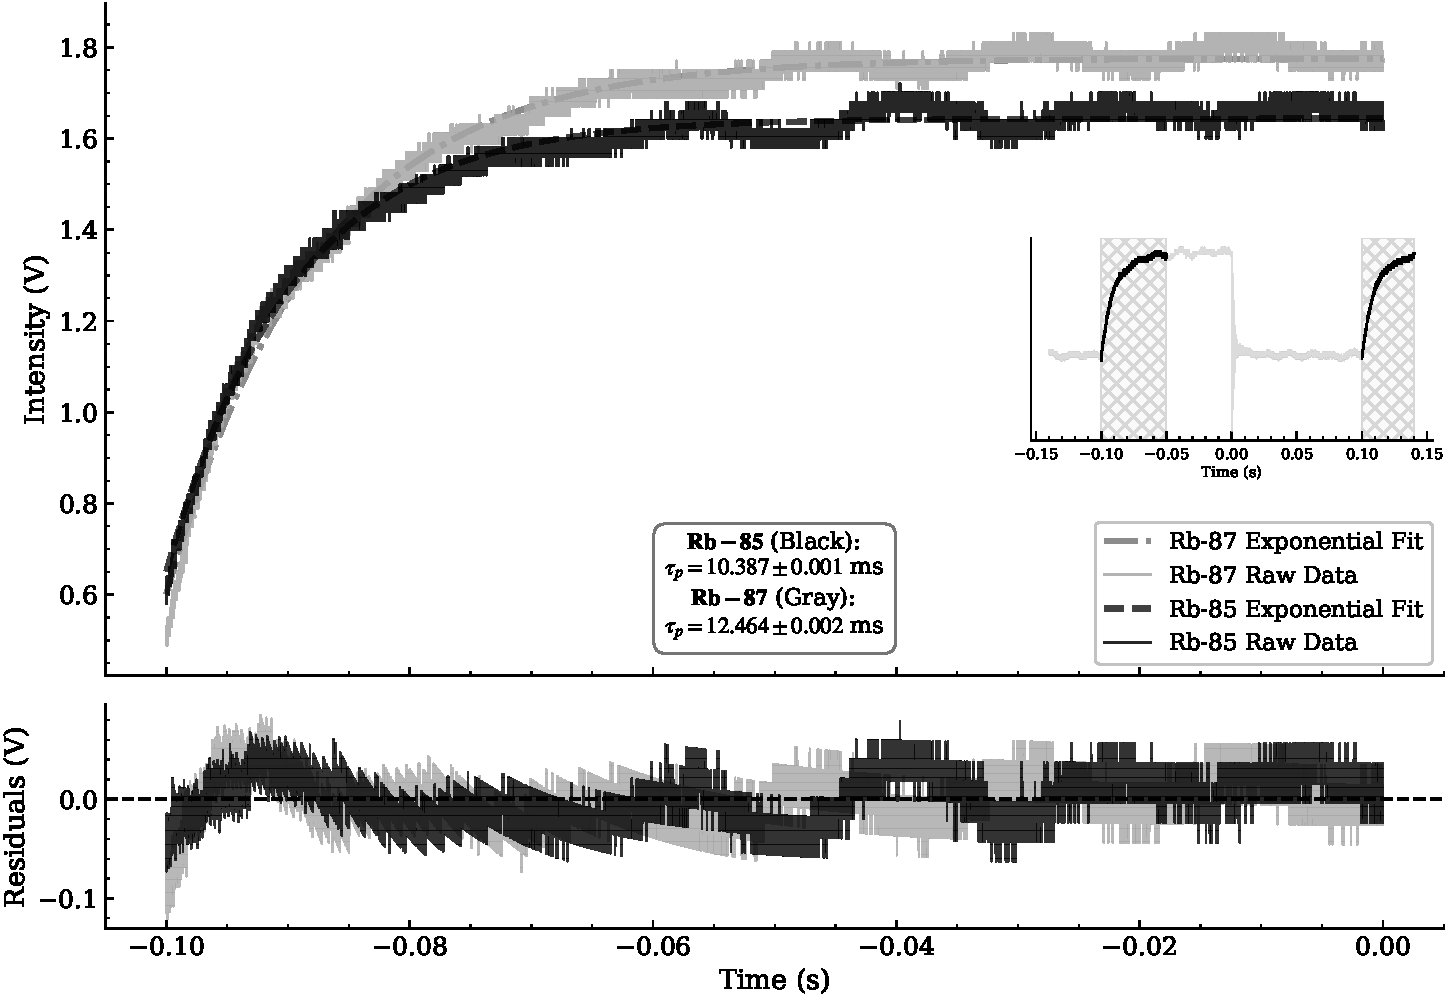
\includegraphics[width=0.9\linewidth]{figures/4d_Optical_Pumping_Recovery_85_87_2VPP.pdf}
  \caption{Optical-pumping recovery curves (upper) and fit residuals
    (lower) for $^{85}$Rb (left) and $^{87}$Rb (right) at
    $V_{\mathrm{pp}} = \SI{2}{\volt}$. Dashed lines: best-fit
    Eq.~\eqref{eq:op_model}.}
  \label{fig:optical_pumping}
\end{figure}

A consistent observation across all six data sets is
$\tau_p^{87} > \tau_p^{85}$. Two channel-strength factors favour faster
pumping in $^{85}$Rb: the dominant pumping channel
$F\!=\!3\to F'\!=\!3$ in $^{85}$Rb has a relative line strength of 0.972
(vs.\ 0.625 for $F\!=\!2\to F'\!=\!2$ in $^{87}$Rb), and the
``bottleneck'' sublevel $|F\!=\!3,m_F\!=\!-3\rangle$ in $^{85}$Rb
(absorption rate 0.243) pumps faster than
$|F\!=\!2,m_F\!=\!-2\rangle$ in $^{87}$Rb (0.208). A full
Franzen--Emslie rate-equation simulation tracking all ground-state
sublevels (8 for $^{87}$Rb, 12 for $^{85}$Rb) with transition
probabilities computed from Clebsch--Gordan coefficients predicts
$\tau_p^{87}/\tau_p^{85} = 1.164$, within $3\%$ of our measured ratio
$1.20005(22)$ at $V_{\mathrm{pp}} = \SI{2}{\volt}$.

Figure~\ref{fig:tau_vs_rf} collects $\tau_p$ versus $V_{\mathrm{pp}}$ for
both isotopes. $\tau_p$ should depend on the optical pumping rate (lamp
intensity) rather than on the RF amplitude, which governs only the
depumping dynamics. The data are consistent with this expectation --
there is no strong systematic trend with $V_{\mathrm{pp}}$ -- though the
scatter is non-negligible given only three voltage settings per isotope.

\begin{figure}[ht]
  \centering
  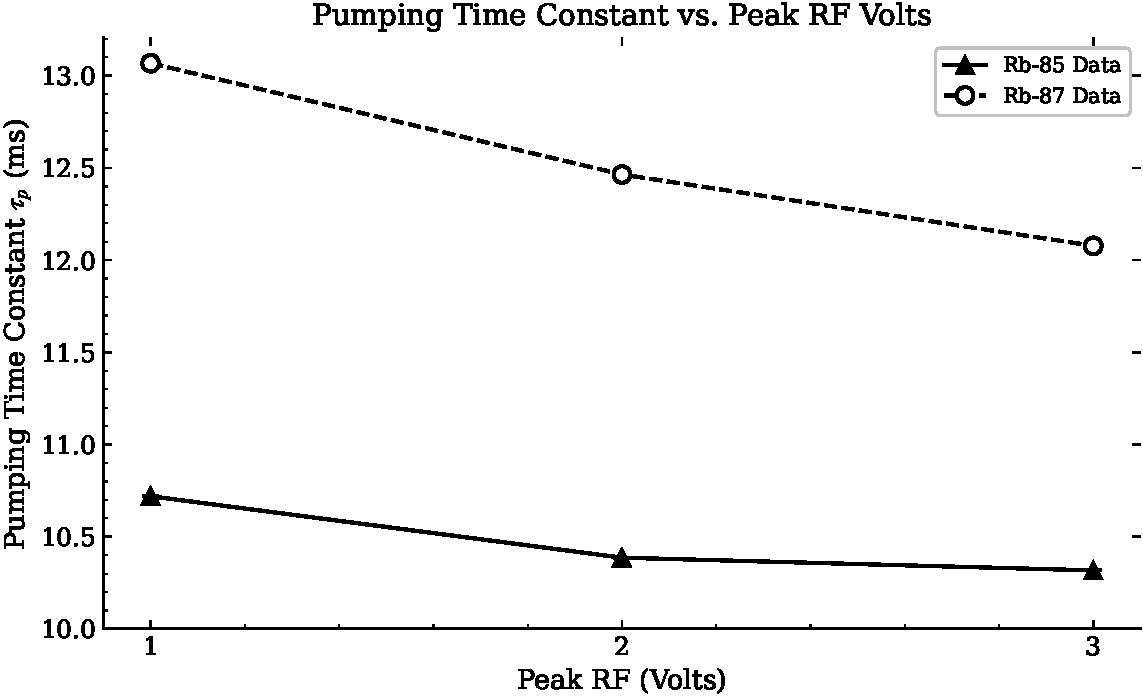
\includegraphics[width=0.7\linewidth]{figures/4d_Pumping_Time_Constant_vs_Peak_RF.pdf}
  \caption{Optical-pumping time constant $\tau_p$ as a function of peak
    RF voltage for $^{85}$Rb and $^{87}$Rb.}
  \label{fig:tau_vs_rf}
\end{figure}

\subsection{Rabi oscillations (ringing effect)}\label{sec:ringing}
The ringing region ($t \in [0.5,3.0]\,\mathrm{ms}$ after the RF onset)
was fit to
\begin{equation}
  V(t) = A\,e^{-\Gamma t}\sin(2\pi f_R t + \phi) + C.
  \label{eq:damped_sine}
\end{equation}
The first \SI{0.5}{\milli\second} was excluded because the initial spike
lacks a well-defined oscillation peak; omitting it improves both fit
stability and accuracy. Figure~\ref{fig:ringing_fit} shows the
representative fit: $f_R = 3035.062(80)\,\si{\hertz}$ with damping
$\Gamma = 723.62(48)\,\si{\per\second}$. The residuals carry a slow
${\sim}\SI{1}{\milli\second}$ modulation with ${\sim}\SI{0.05}{\volt}$
amplitude, attributable to the \SI{60}{\hertz} pickup of
Section~\ref{sec:fft}, beat frequencies between Rabi oscillations of
different $m_F$-sublevel pairs (whose transition matrix elements differ),
or a combination.

\begin{figure}[ht]
  \centering
  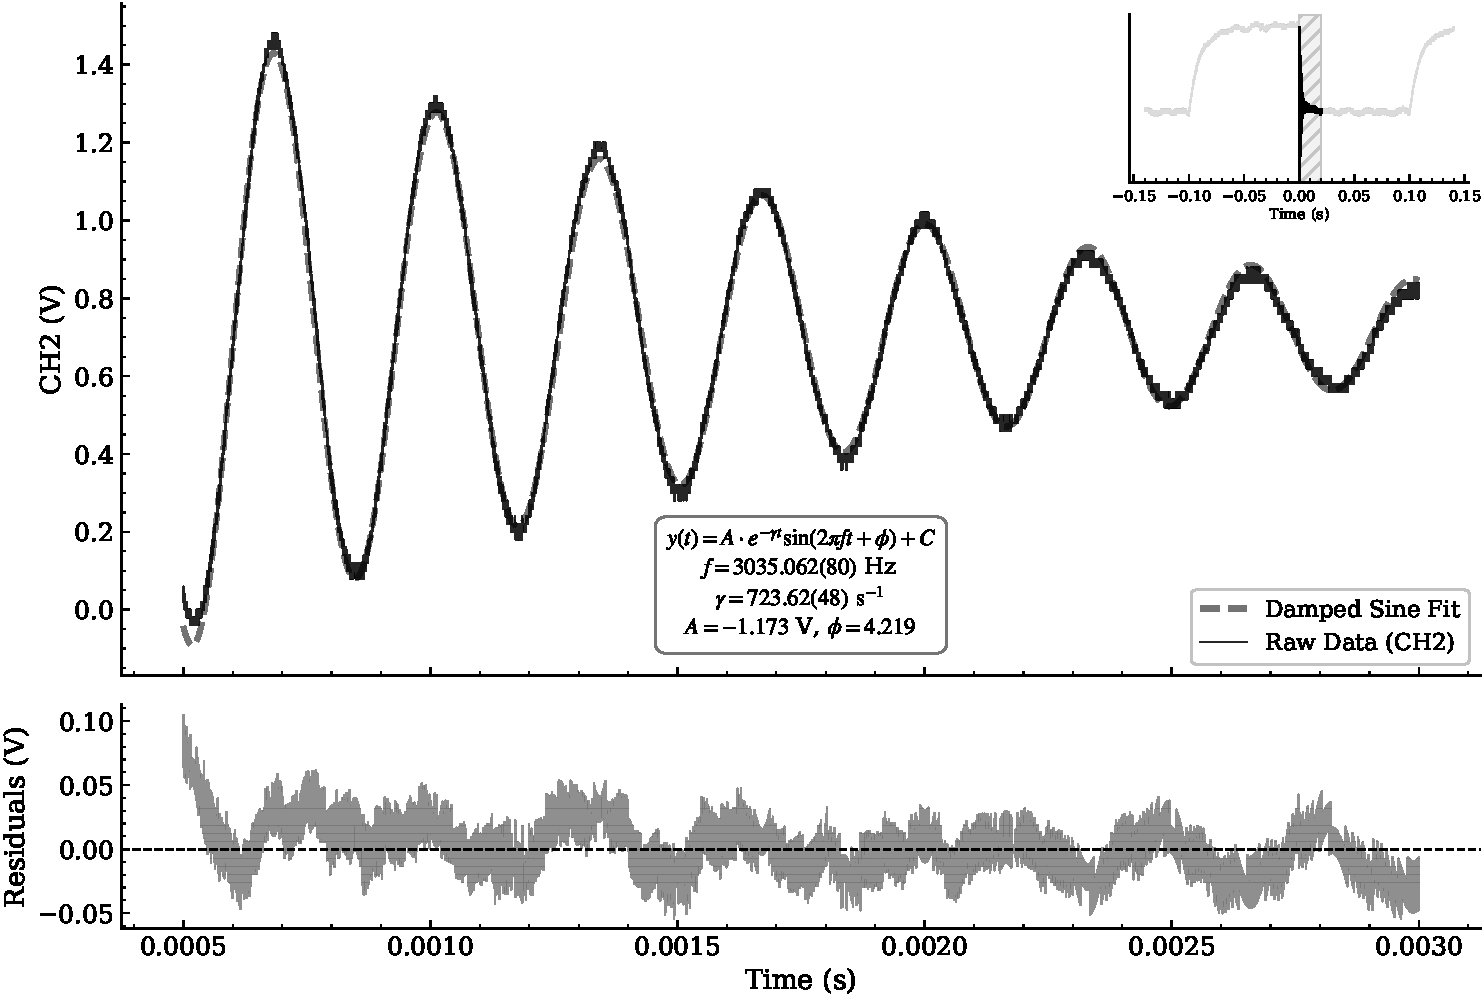
\includegraphics[width=0.9\linewidth]{figures/4d_CH2_Ringing_Fit_with_Residuals.pdf}
  \caption{Damped-sinusoid fit to the ringing transient (upper) and
    residuals (lower) for $^{85}$Rb at $V_{\mathrm{pp}} = \SI{2}{\volt}$.
    Fitted Rabi frequency $f_R = 3035.062(80)\,\si{\hertz}$;
    damping $\Gamma = 723.62(48)\,\si{\per\second}$.}
  \label{fig:ringing_fit}
\end{figure}

At resonance, $T = 1/(\gamma B_{\mathrm{rf}})$ and $B_{\mathrm{rf}}
\propto V_{\mathrm{rf}}$, so we expect
\begin{equation}
  T = k/V_{\mathrm{rf}} + T_0
  \label{eq:period_vs_V}
\end{equation}
with $k$ set by the coil geometry and $\gamma$. An inverse linear
regression over all six data sets is plotted in
Fig.~\ref{fig:period_vs_rf}. Two factors limit the precision: the
combined AFG-2225 amplitude accuracy ($\pm 2\%$ of setting
$\pm\SI{1}{\milli\volt}$) and flatness ($\pm 1\%$ at
\SI{90}{\kilo\hertz}) contribute horizontal error bars of
$\sigma_V = [0.03,\,0.06,\,0.09]\,\mathrm{V}$ at $V_{\mathrm{pp}} =
[1,\,2,\,3]\,\mathrm{V}$; and three voltage points leave effectively one
degree of freedom against the two fit parameters. Additional
measurements at intermediate voltages (e.g.\ 0.5, 1.5, 2.5, 4.0\,V)
would tighten the fit substantially. Despite these limits, both isotopes
clearly exhibit the expected inverse scaling, and the ratio
$T_{87}/T_{85}$ at a given voltage is consistent with the
gyromagnetic-ratio ratio $\gamma_{85}/\gamma_{87}$ predicted by the
rotating-frame analysis.

\begin{figure}[ht]
  \centering
  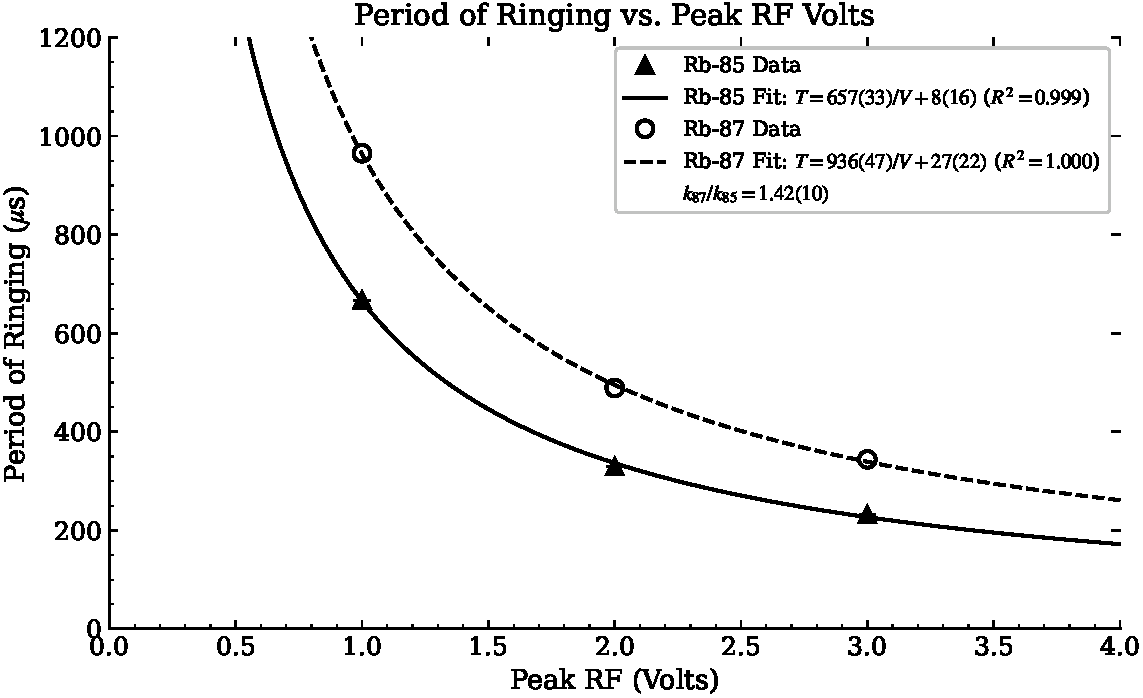
\includegraphics[width=0.7\linewidth]{figures/4d_Period_vs_Peak_RF.pdf}
  \caption{Rabi-oscillation period vs.\ peak RF voltage for $^{85}$Rb and
    $^{87}$Rb. Horizontal error bars include the AFG-2225 amplitude
    accuracy and flatness. Dashed: best-fit Eq.~\eqref{eq:period_vs_V}.}
  \label{fig:period_vs_rf}
\end{figure}
